%\usepackage [ISO-8859-1]{inputenc}
\documentclass[a4paper,12pt,oneside]{amsbook}
\usepackage[T1]{fontenc}
\usepackage{listings}
\usepackage{textcomp}
\usepackage{multicol}
%\usepackage{euler}
%\usepackage{garamond}
\usepackage{hyperref}

\usepackage{newcent}
%\fontfamily{fxm}\selectfont
\usepackage{fancyhdr}
\pagestyle{fancy}
% Detta paket skoter grafiken
%\usepackage[dvips]{graphicx}
\usepackage[pdftex]{graphicx}

\usepackage{amsthm}
\usepackage{amsmath}
\usepackage[swedish]{babel}
% For bortkommentering
\usepackage{verbatim}
% For att slippa indentering av Sections och SubSections
\usepackage{indentfirst}

% Har stalls paragrafindentering och avstand mellan stycken och rader mm
\setlength{\parindent}{0pt}
\setlength{\parskip}{6pt}
\setlength{\baselineskip}{12pt}
% Har definieras sidan
\setlength{\voffset}{-15mm}
\setlength{\hoffset}{-5.5mm}

\setlength{\topmargin}{0mm}
\setlength{\headheight}{10mm}
\setlength{\headsep}{8mm}
\setlength{\footskip}{16mm}

\setlength{\evensidemargin}{0mm}
\setlength{\oddsidemargin}{0mm}

\setlength{\marginparsep}{0mm}
\setlength{\marginparwidth}{0mm}

\setlength{\textwidth}{170mm}
\setlength{\textheight}{230mm}
\setlength{\paperwidth}{210mm}
\setlength{\paperheight}{297mm}
\setlength{\headwidth}{170mm}
% Huvud och Fot
%\fancypagestyle{}{
\fancyhf{}\fancyhead[c]{\small{\textit{Programmeringsolympiaden Kvalificering 2022}}}
\fancyfoot[c]{\thepage}
\renewcommand{\headrulewidth}{0.4pt}
\renewcommand{\footrulewidth}{0.4pt}
\newenvironment{lista}
{\begin{itemize}
\setlength{\parindent}{0pt}
\setlength{\itemsep}{6pt}}
{\end{itemize}}
% Uppgifter
\newcounter{probnr}
\newenvironment{tal}{%
\begin{list}
%{\textbf{\arabic{section}.\arabic{probnr}}} {\usecounter{probnr}
{\textbf{\arabic{probnr}}} {\usecounter{probnr}
\setlength{\leftmargin}{0mm}
\setlength{\rightmargin}{0mm}
\setlength{\labelwidth}{-1mm}
\setlength{\labelsep}{1mm}}
\setlength{\itemsep}{6pt}
}{\end{list}}
% Definition av avsnitt: FAKTA, EXEMPEL, PASTAENDE
\newtheorem{fakta}{Fakta}
\newtheorem{exempel}{Exempel}
\newtheorem{problem}{Problem}
%
\newtheoremstyle{test}% NAME
{20pt}      % ABOVESPACE
{10pt}      % BELOWSPACE
{\sffamily} % BODYFONT
{0pt}       % INDENT
{\scshape}  % HEADFONT
{}          % HEADPUNCT
{\newline}  % HEADSPACE
{}          % CUSTOM-HEAD-SPEC

\theoremstyle{test}
\newtheorem{program}{Program}
\newcommand{\sv}[1]{\textsc{#1}}            % Sma versaler
\newcommand{\fe}[1]{\textbf{#1}}            % FET
\newcommand{\ku}[1]{\textit{#1}}            % KURSIV
\newcommand{\cu}[1]{\texttt{#1}}            % Courier
\newcommand{\sk}[1]{\texttt{#1}}            % Courier
\newcommand{\rubrik}[1]{\begin{center}\sf\huge{#1}\normalsize\rm\end{center}}
\begin{document}
%\DeclareGraphicsExtensions{.jpg,.pdf,.mps,.png,.eps}


\thispagestyle{fancy}
\lstset{basicstyle=\ttfamily,
  breaklines=true}
% ----------------------------------------------------

\begin{center}
\Huge{Programmeringsolympiaden 2022}
\end{center}
\vspace{-1.2cm} 
\specialsection*{Rules}
\begin{lista}
\item The contest is \textbf{four hours long}.
  No extension is given for recess or lunch.
  You may use your own computer or one provided by your teacher.
\item The problem set has six tasks to be solved by a computer program in a language of your choice.
\item {\bf Input can be read however you want}, for example by having a dialog with the user (as in the examples in the tasks), or input into a graphical user interface or reading and writing to files. Make sure you and your teacher agree on how to test your program.
\item Solutions are tested with secret test cases.
  Each task normally has 5 cases, each worth 1 point if your program outputs a correct answer within \textbf{3 seconds}.
  No test of the input should be done -- it will always adhere to the specification in the task.
\item Different test cases may have different constraints, for example on the size of the input.
  This will be specified for each task.
  \textbf{Note that this can affect the difficulty of a task.
  It might be easier to get some points on a harder task than full points on an easier task.}
  The information on partial credit is thus very important.
\item Grading should be done on the same or a similar a computer.
  Changes to the source code is forbidden after the contest.
  If the program does not compile, 0 points are awarded on the task.
\item If one of the following happens, that 
  {\em test cases} gives 0 points, but your program is still tested and can receive points on the other test cases.
\begin{lista}
\item The execution time exceeds 3 seconds \vspace{-0.2cm}
\item Execution error (run time error) \vspace{-0.2cm}
\item Incorrect answer \vspace{-0.2cm}
\end{lista}

\item Participation is individual, so no exchange of ideas, files, source code etc is allowed during the contest.
\item Allowed aids: Any written material, material installed on your computer and material available on the Internet.
  It is \ku{not} allowed to actively communicate on the Internet (like chatting or asking questions on a forum), only search for information.
  A calculator is allowed.
\item Your solutions should be handed in as source code files named uppg1...uppg6 with the appropriate extension.
  No regard is given to other files.
  Make sure you hand in the correct version of your programs!
\end{lista}

%De högst placerade i kvalet går vidare till finalen där landslagsplatser till BOI i Sverige och IOI i Japan står på spel.
\begin{center}
\Large Good luck!
\end{center}
%\end{document}

\newpage
\specialsection*{Task 1 -- Sending Posters}

THE HORROR!
For the $1337$'th year in a row, PostNord has increased the postage fees, a serious risk to the olympiad budget.

Each year, the olympiad sends out posters to about $450$ high schools.
A mail consists of three things:
\begin{itemize}
\item an envelope of C4 size ($229\text{ mm} \times 324\text{ mm}$)
\item two posters of A3 size ($297\text{ mm} \times 420\text{ mm}$)
\item an informational letter of A4 size ($210\text{ mm} \times 297\text{ mm}$)
\end{itemize}

It's very important that the letter weighs at most $50$ grams, since the postage fee otherwise becomes twice as high.
For the mail to beat this magical limit the olympiad controls what kinds of paper are used for the three items.
Each kind has a surface weight (weight per area) that is given in $\frac{\text{gram}}{\text{m}^2}$.
Note that the envelope consists of \textbf{two papers glued together} of C4-size, while the surface weights and the above measurements are given for \emph{one paper}.

Write a program that computes the total weight for a letter.
The program should read three integers between $50$ and $200$, the surface weights in $\frac{\text{gram}}{\text{m}^2}$ for the kinds of paper used for the envelope, the posters and the informational letter.
Output a single real number: the weight of a full mail in grams.
-Your answer must be accurate to at least $3$ decimals, i.e. be within $5 \cdot 10^{-4}$ from the right answer.

%Svaret kommer alltid att ha högst $6$ siffror efter decimaltecknet.

\vspace{1cm}

\fe{Example 1}
\begin{verbatim}
Kuvert ? 120
Affisch ? 90
Blad ? 70

Svar: 44.626140
\end{verbatim}

\vspace{1cm}

\fe{Example 2}
\begin{verbatim}
Kuvert ? 150
Affisch ? 200
Blad ? 90

Svar: 77.768100
\end{verbatim}



\newpage
\specialsection*{Task 2 -- Arabic}
It's well known that when writing text in Arabic you write left-to-right.
It's not as known that you never write out short vowels.

With vowels we mean one of the letters \textit{a,e,i,o,u,y}.
A short vowel is defined as a vowel followed by one or two consonants.

Write a program that shows how a sentence should be displayed as if written in Arabic, i.e. from the left to right and without the short vowels of the original sentence present.
The program should ask for the number of words $N$ ($1 \le N \le 5$), and then read $N$ words where each word consists of at most $10$ small letters (\texttt{a} to \texttt{z}).


\fe{Grading:} For $2$ points, there will be no short vowels in the sentence.

\vspace{1cm}



\fe{Example 1}
\begin{verbatim}
Antal ord ? 4
Mening ? hej vad heter du

Svar: ud reteh dav jeh
\end{verbatim}

\fe{Explanation: } There are no short vowels.

\vspace{1cm}

\fe{Example 2}
\begin{verbatim}
Antal ord ? 1
Mening ? leende

Svar: ednel
\end{verbatim}

\fe{Explanation: } The second \emph{e} in the word \emph{leende} is a short vowel, so it's omitted. Note that the first \emph{e} remains, since it's not a short vowel in the first sentence.

\vspace{1cm}

\fe{Example 3}
\begin{verbatim}
Antal ord ? 5
Mening ? po ar en trevlig tavling

Svar: gnlvt gilvrt ne ra op
\end{verbatim}


\newpage
\specialsection*{Task 3 -- Green card}

To rope climb, you need two people; one that climbs, and one that stands on the ground to secure the rope in case the climber falls down.
To secure the rope, you must first have taken a course to receive a green card.
However, you don't need a green card to climb.
To climb a wall, including tying the rope into both the climber and the person securing the climber takes exactly $10$ minutes.
There are many climbing walls, so any number of people can climb at the same time (but must be secured by different people).

A group of friends has $N$ people with a green card and $M$ people without, where $2 \le N \le 400\,000\,000$ and $0 \le M \le 400\,000\,000$.
How many minutes does it take for everyone to climb the wall once?

\fe{Grading:}\\
For $1$ point $M = 0$ (but $N$ can be large).\\
For $1$ additional point $N = 2$ (but $M$ can be large).\\
For $2$ additional points $M,N \le 100$.


\vspace{0.5cm}

\fe{Example 1}
\begin{verbatim}
Antal med grönt kort, N  ? 2
Antal utan grönt kort, M ? 0

Svar: 20
\end{verbatim}

\fe{Explanation:} There are two people, both with green cards.
One of them climbs first while the other one secures, and then they switch roles.

\vspace{0.5cm}

\fe{Example 2}
\begin{verbatim}
Antal med grönt kort, N  ? 2
Antal utan grönt kort, M ? 2

Svar: 30
\end{verbatim}

\fe{Explanation:} There are four people, of which two have a green card.
The two people with a card can climb during the first $20$ minutes (as in the first example).
Afterwards the other two people can climb at the same time.

\vspace{0.5cm}

\fe{Example 3}
\begin{verbatim}
Antal med grönt kort, N  ? 3
Antal utan grönt kort, M ? 3

Svar: 30
\end{verbatim}

\fe{Explanation:} There are six people, of which three have a green card.
One way in which they can climb in $30$ minutes is for two people to always climb at the same time; one with a green card and one without.


\newpage
\specialsection*{Task 4 -- The tired painter}

Ilad Rodavlas has painted his whole life but is now getting tired of his job.

But one day when painting a floor, divided into $N \times N$ squares, he gets an idea.
``What if a robot could do my job for me!'' he asked.
There are two problems with this idea.
First, the robot can only move in a straight line, so it can only paint a row or a column with the same color.
Secondly, Ilad can't program.
Can you help him?

Ilad has an image that shows exactly how the floor should look.
In the beginning, the floor is unpainted.
Write a program to give instructions to the robot for how it should paint the floor.
To not waste paint, it must not paint the same row or column more than once.

%För att inte slösa på färg får roboten inte måla en rad eller kolumn, om samtliga rutor i raden eller kolumnen målas över (möjligtvis av samma färg) senare.
%Den får heller inte måla en rad eller kolumn om alla rutor i raden eller kolumnen redan har den tiltänkta färgen.

The program should read an integer $1 \leq N \leq 9$, the number of rows and columns of the floor.
Then it should read $N$ lines with $N$ characters, a dot ($.$) for an unpainted square, $S$ for a black square and $V$ for a white square.
It will always be possible to paint the floor with this pattern.

Output a text string with the rows and columns the robot should paint, in order.
Rows are denoted by the numbers $1$, $2$, $\dots$ and columns with the letters $A$, $B$, $\dots$ (see the figure).
Then output a string of the same length with the colors the robot should paint, using \texttt{V} for white and \texttt{S} for black.

\fe{Grading:} For $2$ points $N \le 4$.
\setlength\columnsep{20pt}
\begin{multicols}{3}

\fe{Example 1}
%\begin{lstlisting}
\begin{verbatim}
N ? 4
Rad 1 ? ..S.
Rad 2 ? VVSV
Rad 3 ? ..S.
Rad 4 ? ..S.

Ordning: 2C
Färger : VS


\end{verbatim}
%\end{lstlisting}
\vfill
\columnbreak

\fe{Example 2}
\begin{verbatim}
N ? 5
Rad 1 ? VVVVV
Rad 2 ? ..S.S
Rad 3 ? VVVVS
Rad 4 ? VVVVV
Rad 5 ? ..S.S

Ordning: C3E41
Färger : SVSVV

\end{verbatim}
\vfill
\columnbreak

\fe{Example 3}
\begin{verbatim}
N ? 6
Rad 1 ? VVVVVV
Rad 2 ? VVVSVV
Rad 3 ? VVVSVV
Rad 4 ? V.VSV.
Rad 5 ? SSSSSS
Rad 6 ? V.VSV.

Ordning: 32EDCA51
Färger : VVVSVVSV
\end{verbatim}

\vfill
\end{multicols}
\begin{multicols}{2}
\begin{center}
  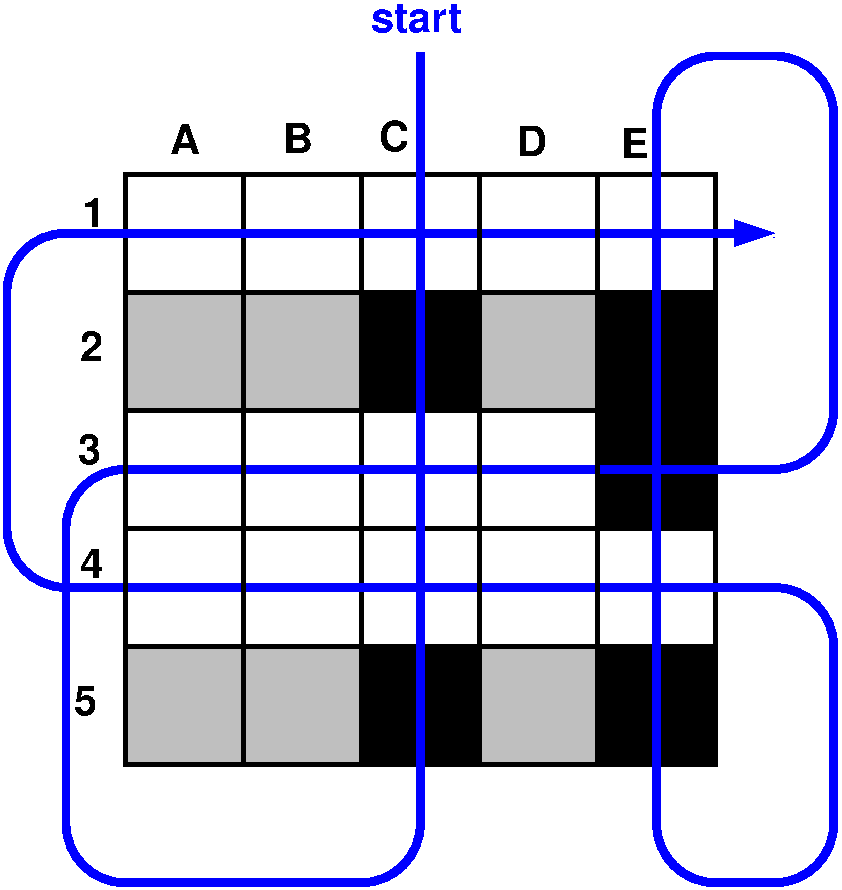
\includegraphics[width=5cm]{../skolkval/dentrottemalaren/problem_statement/golv.pdf}
\end{center}
\columnbreak
~\\ 
    \emph{The arrow shows a possible way of painting in the second example. Gray color denotes unpainted squares. \textbf{There are several different solutions to the example cases.}
    For example you can switch which of the rows $1$ and $4$ you start with in example 2.
    }
\vfill
\end{multicols}

\newpage
\specialsection*{Task 5 -- Short vowels}

Solving algorithmic problems is difficult, but something that's often harder is preparing test data.
Take \textit{Arabic} for example.
The jury spent hours of intensive work to construct masterpieces such as the test case \texttt{hej vad heter du}.

A question we had to answer was: how do you make text strings that don't contain short vowels?
If you read the task \textit{Arabic} you might remember that a short vowel is a vowel followed by two consonants.
In the word \texttt{tall} the a is a short vowel, while the word \texttt{potatis} lacks short vowels.
For simplicity, we consider \textit{a, e, i, o, u, y} to be vowels.

One way of making such words is to start with a word and then remove letters from it.
Starting with the word \texttt{potatis} we might get \texttt{ptais} for example.
But if the word instead became \texttt{otats} we unfortunately got a short vowel.

Given a word, compute the number of ways letters can be removed such that the remaining word doesn't contain any short vowels.
It's allowed to not remove any letters (in the second example, this contributes $1$ to the answer).
However, it's not allowed to remove all letters.
If the same word is formed by removing different sets of letters, they are counted separately (in the first example there are two ways of making \texttt{tal}, by removing either the first or second \texttt{l}).

Your program should read a word with of length at most $50$ containing only letters \texttt{a-z}.
It should output an integer, the number of ways to remove letters such that the remainder has no short vowels.
Note that the answer might not fit in a $32$-bit integer in the latter test cases.

\fe{Grading:}\\
For $1$ point all letters in the word are the same.\\
For $2$ additional points the word contains at most $10$ letters.


\vspace{1cm}

\fe{Example 1}
\begin{verbatim}
Ord ? tall

Svar: 13
\end{verbatim}

\vspace{1cm}

\fe{Example 2}
\begin{verbatim}
Ord ? potatis

Svar: 107
\end{verbatim}


\newpage
\specialsection*{Task 6 -- Mountain Range}


\noindent
Torunn lives in a mountain range consisting of an $n \times m$ grid with a house in each square.
She lives in the top left square of the grid.
Unfortunately an annoying neighbor just moved in, so Torunn wants to sell her house and move.
First, she needs to figure our how much her house is worth.

Each square in the grid has a given elevation.
All elevations are different, so let us for simplicity assume that they are $1, 2, 3, \dots, n\cdot m$.
Houses at higher elevations are worth more, so she wants to figure out the elevation of her house.
She therefore went to every square and figured out how many adjacent squares are at a lower elevation.
Two squares are adjacent if they share a side (meaning squares not at the edges of the grid has $4$ adjacent squares).

Write a program that, given the information Torunn collected, finds the smallest and greatest possible elevation of her house.

The program should read two integers $n$ and $m$ ($1 \leq n,m \leq 8$), the number of rows and columns in the grid.
Afterwards it should read $n$ lines containing an $m$ character string.
These lines contains the information Torunn collected, with each digit denoting the number of adjacent square at a lower elevation.
It's guaranteed that the elevations $1, 2, \dots, n\cdot m$ can be assigned to the squares in a manner consistent with these values.
Note that the values are always between $0$ and $4$.

Output two integers; the smallest and greatest possible elevation of the house in the top left square of the grid.

\fe{Grading}\\
For $1$ point, $n = 1$.\\
For $1$ additional point, $n = m = 3$.\\
For $1$ additional point, $n = m = 4$.\\

\vspace{0.5cm}

\setlength\columnsep{30pt}
\begin{multicols}{2}

\fe{Example 1}
\begin{verbatim}
n ? 2
m ? 3
Rad 1 ? 122
Rad 2 ? 101

Svar: 3 4
\end{verbatim}

\vspace{0.5cm}
\fe{Example 2}
\begin{verbatim}
n ? 1
m ? 4
Rad 1 ? 0111

Svar: 1 1
\end{verbatim}

\vfill\columnbreak
\begin{center}
  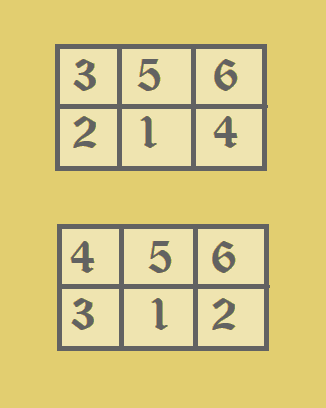
\includegraphics[width=5cm]{../skolkval/bergskedja/problem_statement/berg_sample}\\
  \emph{Two possible elevation maps for example $1$.}
\end{center}
\vfill
\end{multicols}



\end{document}

